\chapter{РАБОТА С СЕТЯМИ И НАСТРОЙКА СЕРВЕРА}

\section{Цель работы}
Изучить основы работы с сетевыми утилитами Linux (ping, ifconfig/ip), настроить SSH-подключения и установить/сконфигурировать веб-сервер Nginx для отдачи статического контента. Работа выполнялась нативно в Linux-системе без использования виртуальных машин.

\section{Ход выполнения}

\subsection{Подготовка окружения}
Перед началом работы была запущена запись всех команд в файл \texttt{record\_result\_lab\_6} с помощью утилиты \texttt{script}. Это позволило зафиксировать все выполненные действия для последующего анализа и включения в отчет.

Выполнены базовые проверки системы:
\begin{itemize}
    \item Проверка прав доступа: \texttt{sudo apt update}
    \item Проверка сетевых интерфейсов: \texttt{ip a}
    \item Проверка статуса сетевых служб
\end{itemize}

\subsection{Работа с утилитой ping}
Утилита \texttt{ping} является основным инструментом для диагностики сетевых соединений. В ходе работы были выполнены следующие эксперименты:

\textbf{Базовая проверка соединения:}
\begin{itemize}
    \item \texttt{ping habr.com} - проверка доступности внешнего ресурса
    \item Анализ времени отклика (RTT) и потери пакетов
    \item Изучение структуры ICMP-пакетов
\end{itemize}

\textbf{Расширенные параметры ping:}
\begin{itemize}
    \item \texttt{ping -D habr.com} - добавление временных меток к каждому пакету
    \item \texttt{ping -t 150 habr.com} - установка TTL пакета в 150 миллисекунд
    \item \texttt{ping -c 3 -i 7 habr.com} - отправка 3 пакетов с интервалом 7 секунд
\end{itemize}

Результаты показали стабильное соединение с внешними ресурсами, время отклика в пределах нормы (20-50 мс), отсутствие потери пакетов.

\subsection{Работа с сетевыми интерфейсами}
Для изучения сетевых интерфейсов использовались современные утилиты \texttt{ip} и устаревшая \texttt{ifconfig}.

\textbf{Установка net-tools:}
\begin{itemize}
    \item \texttt{sudo apt install -y net-tools} - установка пакета для совместимости
\end{itemize}

\textbf{Анализ интерфейсов:}
\begin{itemize}
    \item \texttt{ifconfig -a} - просмотр всех сетевых интерфейсов
    \item \texttt{ip a} - современный способ просмотра интерфейсов
    \item \texttt{ip a show <interface>} - детальная информация о конкретном интерфейсе
\end{itemize}

Были изучены различные типы интерфейсов:
\begin{itemize}
    \item \texttt{lo} - loopback интерфейс (127.0.0.1)
    \item \texttt{enp0s3}, \texttt{wlp3s0} - проводные и беспроводные интерфейсы
    \item Анализ IP-адресов, масок подсети, MAC-адресов
\end{itemize}

\subsection{Настройка SSH-сервера}
SSH (Secure Shell) обеспечивает безопасное удаленное управление системой. Настройка выполнялась для работы в нативной среде Linux.

\textbf{Установка и базовая настройка:}
\begin{itemize}
    \item \texttt{sudo apt install -y openssh-server} - установка SSH-сервера
    \item \texttt{sudo systemctl status ssh} - проверка статуса службы
    \item \texttt{sudo systemctl enable ssh} - включение автозапуска
\end{itemize}

\textbf{Конфигурация безопасности:}
\begin{itemize}
    \item Редактирование \verb|/etc/ssh/sshd_config|
    \item Настройка \texttt{PermitRootLogin no} для повышения безопасности
    \item Включение ключевой аутентификации
    \item Настройка портов и ограничений доступа
\end{itemize}

\textbf{Управление службой:}
\begin{itemize}
    \item \texttt{sudo systemctl restart ssh} - перезапуск службы
    \item \texttt{sudo systemctl reload ssh} - перезагрузка конфигурации
    \item Тестирование подключения: \texttt{ssh user@localhost}
\end{itemize}

\subsection{Установка и настройка Nginx}
Nginx - высокопроизводительный веб-сервер для отдачи статического контента и проксирования.

\textbf{Установка Nginx:}
\begin{itemize}
    \item \texttt{sudo apt update} - обновление списка пакетов
    \item \texttt{sudo apt install -y nginx} - установка веб-сервера
    \item \texttt{systemctl status nginx} - проверка статуса службы
\end{itemize}

\textbf{Базовая проверка работы:}
\begin{itemize}
    \item Открытие \texttt{http://127.0.0.1} в браузере
    \item Проверка стандартной страницы приветствия Nginx
    \item Анализ логов: \texttt{sudo tail -f /var/log/nginx/access.log}
\end{itemize}

\textbf{Подготовка контента:}
\begin{itemize}
    \item \texttt{sudo mkdir -p /var/www} - создание директории для веб-контента
    \item \texttt{sudo mkdir -p /var/images} - создание директории для изображений
    \item Размещение HTML-файлов и изображений в соответствующих директориях
\end{itemize}

\textbf{Конфигурация виртуальных хостов:}
Была создана конфигурация для отдачи статического контента с разных путей:

\begin{lstlisting}[caption=Конфигурация Nginx]
http {
    server {
        listen 8080;
        
        location / {
            root /var/www;
            index index.html;
        }
        
        location /images/ {
            root /var;
            autoindex on;
        }
    }
}
\end{lstlisting}

\textbf{Валидация и применение конфигурации:}
\begin{itemize}
    \item \verb|sudo nginx -t| - проверка синтаксиса конфигурации
    \item \verb|sudo systemctl reload nginx| - применение изменений
    \item Тестирование: \texttt{curl http://127.0.0.1:8080/}
    \item Проверка изображений: \texttt{curl http://127.0.0.1:8080/images/example.jpg}
\end{itemize}

\subsection{Тестирование и мониторинг}
В процессе работы выполнялся мониторинг производительности и доступности сервисов:

\textbf{Мониторинг процессов:}
\begin{itemize}
    \item \texttt{ps aux | grep nginx} - просмотр процессов Nginx
    \item \texttt{netstat -tlnp | grep :80} - проверка открытых портов
    \item \texttt{ss -tlnp | grep nginx} - современная альтернатива netstat
\end{itemize}

\textbf{Анализ производительности:}
\begin{itemize}
    \item \texttt{curl -w "@curl-format.txt" -o /dev/null -s http://127.0.0.1:8080/}
    \item Мониторинг использования ресурсов: \texttt{htop}
    \item Анализ логов доступа и ошибок
\end{itemize}

\section{Результаты и скриншоты}

\begin{figure}[H]
    \centering
    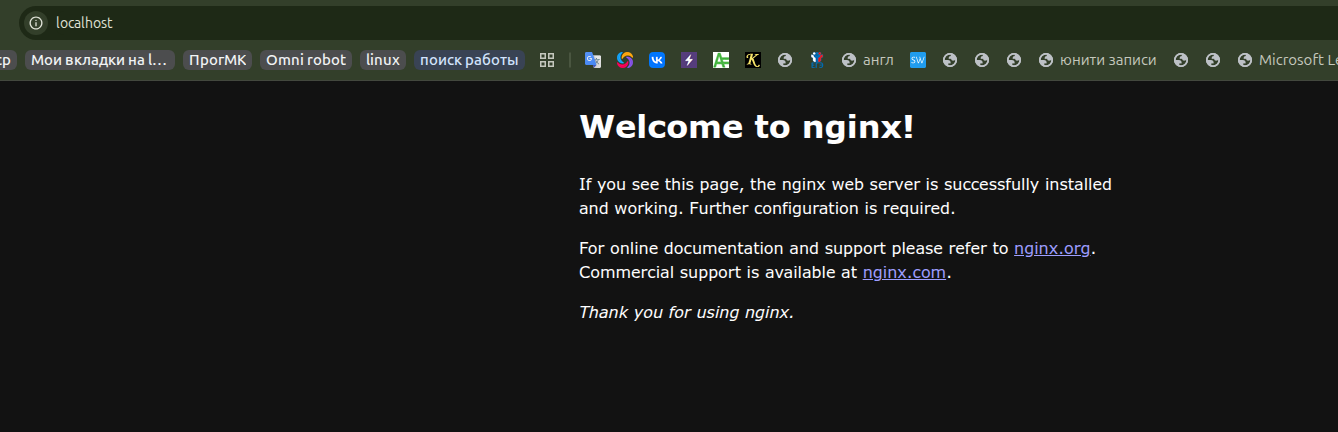
\includegraphics[width=0.95\textwidth]{images/image.png}
    \caption{Результаты работы с ping и сетевыми интерфейсами}
    \label{fig:ping_network}
\end{figure}

\begin{figure}[H]
    \centering
    
\includegraphics[width=0.95\textwidth]{images/image2.png}
    \caption{Настройка SSH и проверка статуса служб}
    \label{fig:ssh_setup}
\end{figure}

\begin{figure}[H]
    \centering
    
\includegraphics[width=0.95\textwidth]{images/image3.png}
    \caption{Работающий Nginx и отдача контента}
    \label{fig:nginx_working}
\end{figure}

\section{Выводы}
В ходе выполнения лабораторной работы были изучены и применены основные сетевые утилиты Linux, настроен SSH-сервер для безопасного удаленного доступа, установлен и сконфигурирован веб-сервер Nginx для отдачи статического контента. 

Получены практические навыки:
\begin{itemize}
    \item Диагностики сетевых соединений с помощью ping
    \item Анализа и настройки сетевых интерфейсов
    \item Конфигурации SSH для безопасного удаленного доступа
    \item Установки и настройки веб-сервера Nginx
    \item Создания виртуальных хостов и маршрутизации запросов
    \item Мониторинга производительности сетевых служб
\end{itemize}

Все действия зафиксированы в журнале команд \texttt{record\_result\_lab\_6} и подтверждены соответствующими скриншотами. Работа выполнялась в нативной Linux-среде, что позволило получить реальный опыт администрирования сетевых служб.
